\graphicspath{{images/appendices}}

\section*{Appendices}

\begin{frame}{Variational formulation of Delaunay triangulations (I)}
	\scriptsize 
	\begin{minipage}{0.3\linewidth}
		\centering
		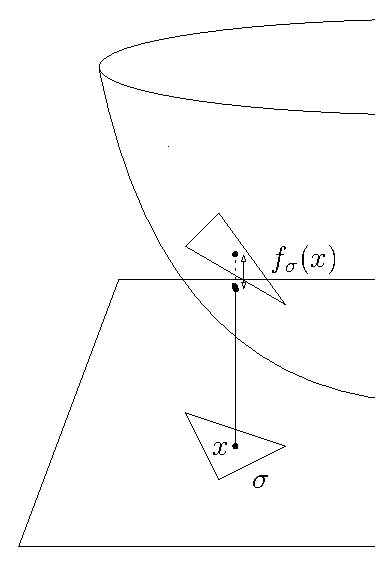
\includegraphics[width=\linewidth]{height_difference}
	\end{minipage}%
	\hfill%
	\begin{minipage}{0.65\linewidth}
		\textbf{Variational characterization} of Delaunay triangulation \cite{musin_ConstructionVoronoiDiagram_2003, chen_OptimalDelaunayTriangulations_2004}
		
		\[
		\begin{aligned}
			f_\sigma : |\sigma| &\to \R\\
			x  &\mapsto f_\sigma(x) \defunder{=} \sum_i \lambda_i(x) \norm{P_i}^2 - \norm{x}^2
		\end{aligned}
		\]
		
		\[
		w_p(\sigma) \defunder{=} \| f_\sigma \|_{p} =  \left(  \int_{|\sigma|} f_\sigma(x)^p dx \right)^{\frac{1}{p}}
		\]
		
		\[
		\Delaunay(\mathbf{P}) = \argmin_{\mathcal{T} \in \mathcal{V}_{\mathbf{P}}} \left(\sum_{\sigma \in \mathcal{T}} w_p(\sigma)^p \right)^{\frac{1}{p}}
		\] where $\mathcal{V}_{\mathbf{P}}$ : set of all triangulations of the convex hull $\CH(\mathbf{P})$.
	\end{minipage}
\end{frame}

\begin{frame}{Variational formulation of Delaunay triangulations (II)}
	\scriptsize

	Equivalent formulation in terms of chains
	\[
		\begin{aligned}
			\norm { \Gamma }_{(p)} : \Cchains_d(K_{\mathbf{P}}) &\to \R\\
			\Gamma &\mapsto \sum_{\sigma \in K^{(d)}} | \Gamma( \sigma)|  w_p(\sigma)^p	
		\end{aligned}
	\]
	
	\begin{block}{\scriptsize Variational formulation (simplicial chains)}
	Denote by $\beta_{\mathbf{P}} \in \Bchains_{d-1}(K_{\mathbf{P}})$ the $(d-1)$-boundary made of the simplices belonging to the boundary of $\mathcal{CH}(\mathbf{P})$. For any $p\in [1, \infty)$, define the chain
	\begin{equation*}
		\Gamma_{\min} \defunder{=} \argmin_{\substack{\Gamma \in \Cchains_{d}(K_{\mathbf{P}})\\
				\partial \Gamma = \beta_{\mathbf{P}}}} \norm{\Gamma}_{(p)}
	\end{equation*}
	The support $|\Gamma_{\min}|$ of $\Gamma_{\min}$ corresponds to all $d$-simplices of the Delaunay triangulation of $\mathbf{P}$.
	\end{block}
\end{frame}

\begin{frame}{Generalizing the total order (I)}
	
\scriptsize
\begin{block}{\scriptsize Weighted distance}
Given two weighted points $(P_1,\mu_1), (P_2,\mu_2) \in \R^d\times \R$ their weighted distance is defined as:
\[
\WDist \left( (P_1,\mu_1), (P_2,\mu_2) \right) \defunder{=} (P_1-P_2)^2 - \mu_1 - \mu_2 
\]
\end{block}

\textbf{Circumweight} (Generalized circumscribed sphere radius)
\[
	\mu_C\left(\sigma \right)  \defunder{=} \min \left\{ \mu \in \R, \exists P \in \R^d, \forall (P_i,\mu_i) \in \sigma, \: \WDist \left(  (P, \mu), (P_i, \mu_i) \right) = 0 \right\}
\]

\textbf{Bounding weight} (Generalized smallest enclosing ball radius)
\[
	\mu_B\left(\sigma \right)  \defunder{=} \min \left\{ \mu \in \R, \exists P \in \R^d, \forall (P_i,\mu_i) \in \sigma, \: \WDist \left(  (P, \mu), (P_i, \mu_i) \right) \leq 0 \right\}
\]

\end{frame}

\begin{frame}{Generalizing the total order (II)}
	\scriptsize
	
	\begin{minipage}{0.6\linewidth}
		\textbf{Minimal face} $\Theta(\sigma)$ verifying: $\mu_B(\Theta(\sigma)) = \mu_B(\sigma)$
		
		\textbf{Sequence of inclusion-increasing faces}
		\begin{eqnarray*}
			\Theta_0(\sigma) & \defunder{=} & \Theta(\sigma) \\
			\Theta_k(\sigma) & \defunder{=} & \argmin_{\substack{\Theta_{k-1}(\sigma) \preceq \tau 	\preceq \sigma\\ \dim{\tau} = \dim{\Theta_{k-1}(\sigma) + 1}}} \mu_C(\tau) \\
			\mu_k(\sigma) &\defunder{=}& \mu_C(\Theta_{k}(\sigma))
		\end{eqnarray*}
	\end{minipage}%
	\begin{minipage}{0.4\linewidth}
		\centering
		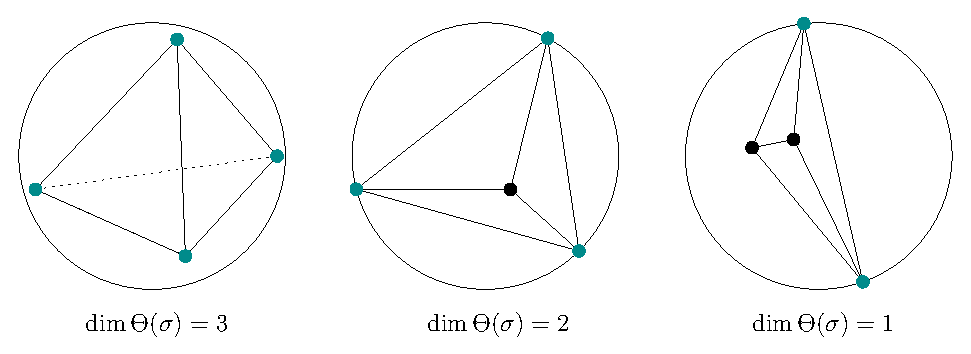
\includegraphics[width=0.95\linewidth]{theta_for_tetra}
	\end{minipage}

	\begin{block}{\scriptsize Generalized total order on $k$-simplices} For $\sigma_1, \sigma_2 \in K^{(d)}$, \[
			\sigma_1 \leq \sigma_2  
			\defunder{\iff}
			\sigma_1 = \sigma_2 \quad \operatorname{or} \quad
			\begin{cases}
				\Krad{0}(\sigma_1) < \Krad{0}(\sigma_2) &\\
				\quad \operatorname{or} &\\
				\exists k\geq 1, \: \Krad{k}(\sigma_1) > \Krad{k}(\sigma_2) &\\ 
				\operatorname{and} \: \forall j, \: 0\leq j < k, \: \Krad{j}(\sigma_1) = \Krad{j}(\sigma_2) &
			\end{cases}
		\]
	\end{block}
\end{frame}

\begin{frame}{Generalizing the total order (III)}
\scriptsize
\begin{theorem}
	Let $\mathbf{P} = \{(P_1, \mu_1) , \ldots, (P_N, \mu_N) \} \subset \R^d \times \R$, with $N \geq d+1$ be in general position and let $K_{\mathbf{P}}$ be the $d$-dimensional full complex  over $\mathbf{P}$. Denote by $\beta_{\mathbf{P}} \in \Bchains_{d-1}(K_{\mathbf{P}})$ the $(d-1)$-boundary made of simplices belonging to the boundary of $\mathcal{CH}(\mathbf{P})$. Define the chain
	\begin{equation*}
		\Gamma_{\min} \defunder{=}  \min_{\LexicographicOrderChain}  \{ \Gamma \in  \Cchains_d(K_{\mathbf{P}}),  \partial \Gamma = \beta_{\mathbf{P}} \}
	\end{equation*}
	The support $|\Gamma_{\min}|$ of  $\Gamma_{\min}$ corresponds to the $d$-simplices of the regular triangulation of $\mathbf{P}$.
\end{theorem}

\end{frame}

\begin{frame}{Non-manifold configurations}
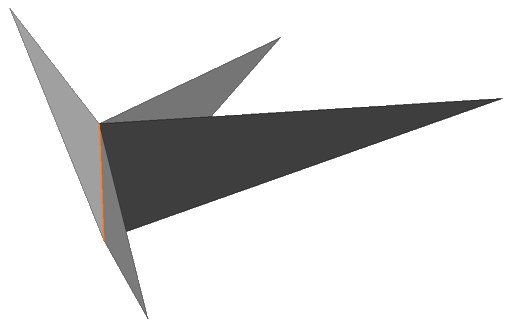
\includegraphics[width=0.5\linewidth]{nonmanifold1}%
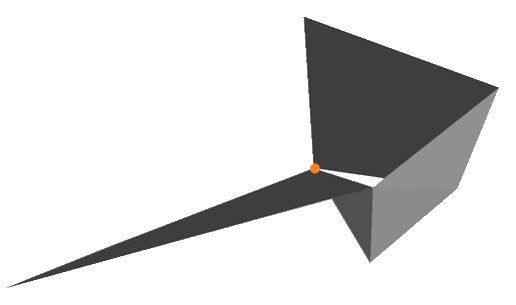
\includegraphics[width=0.5\linewidth]{nonmanifold2}%
\end{frame}

\begin{frame}{Comparison with other methods}
	\scriptsize
	
	\begin{minipage}{0.5\linewidth}
		\centering
		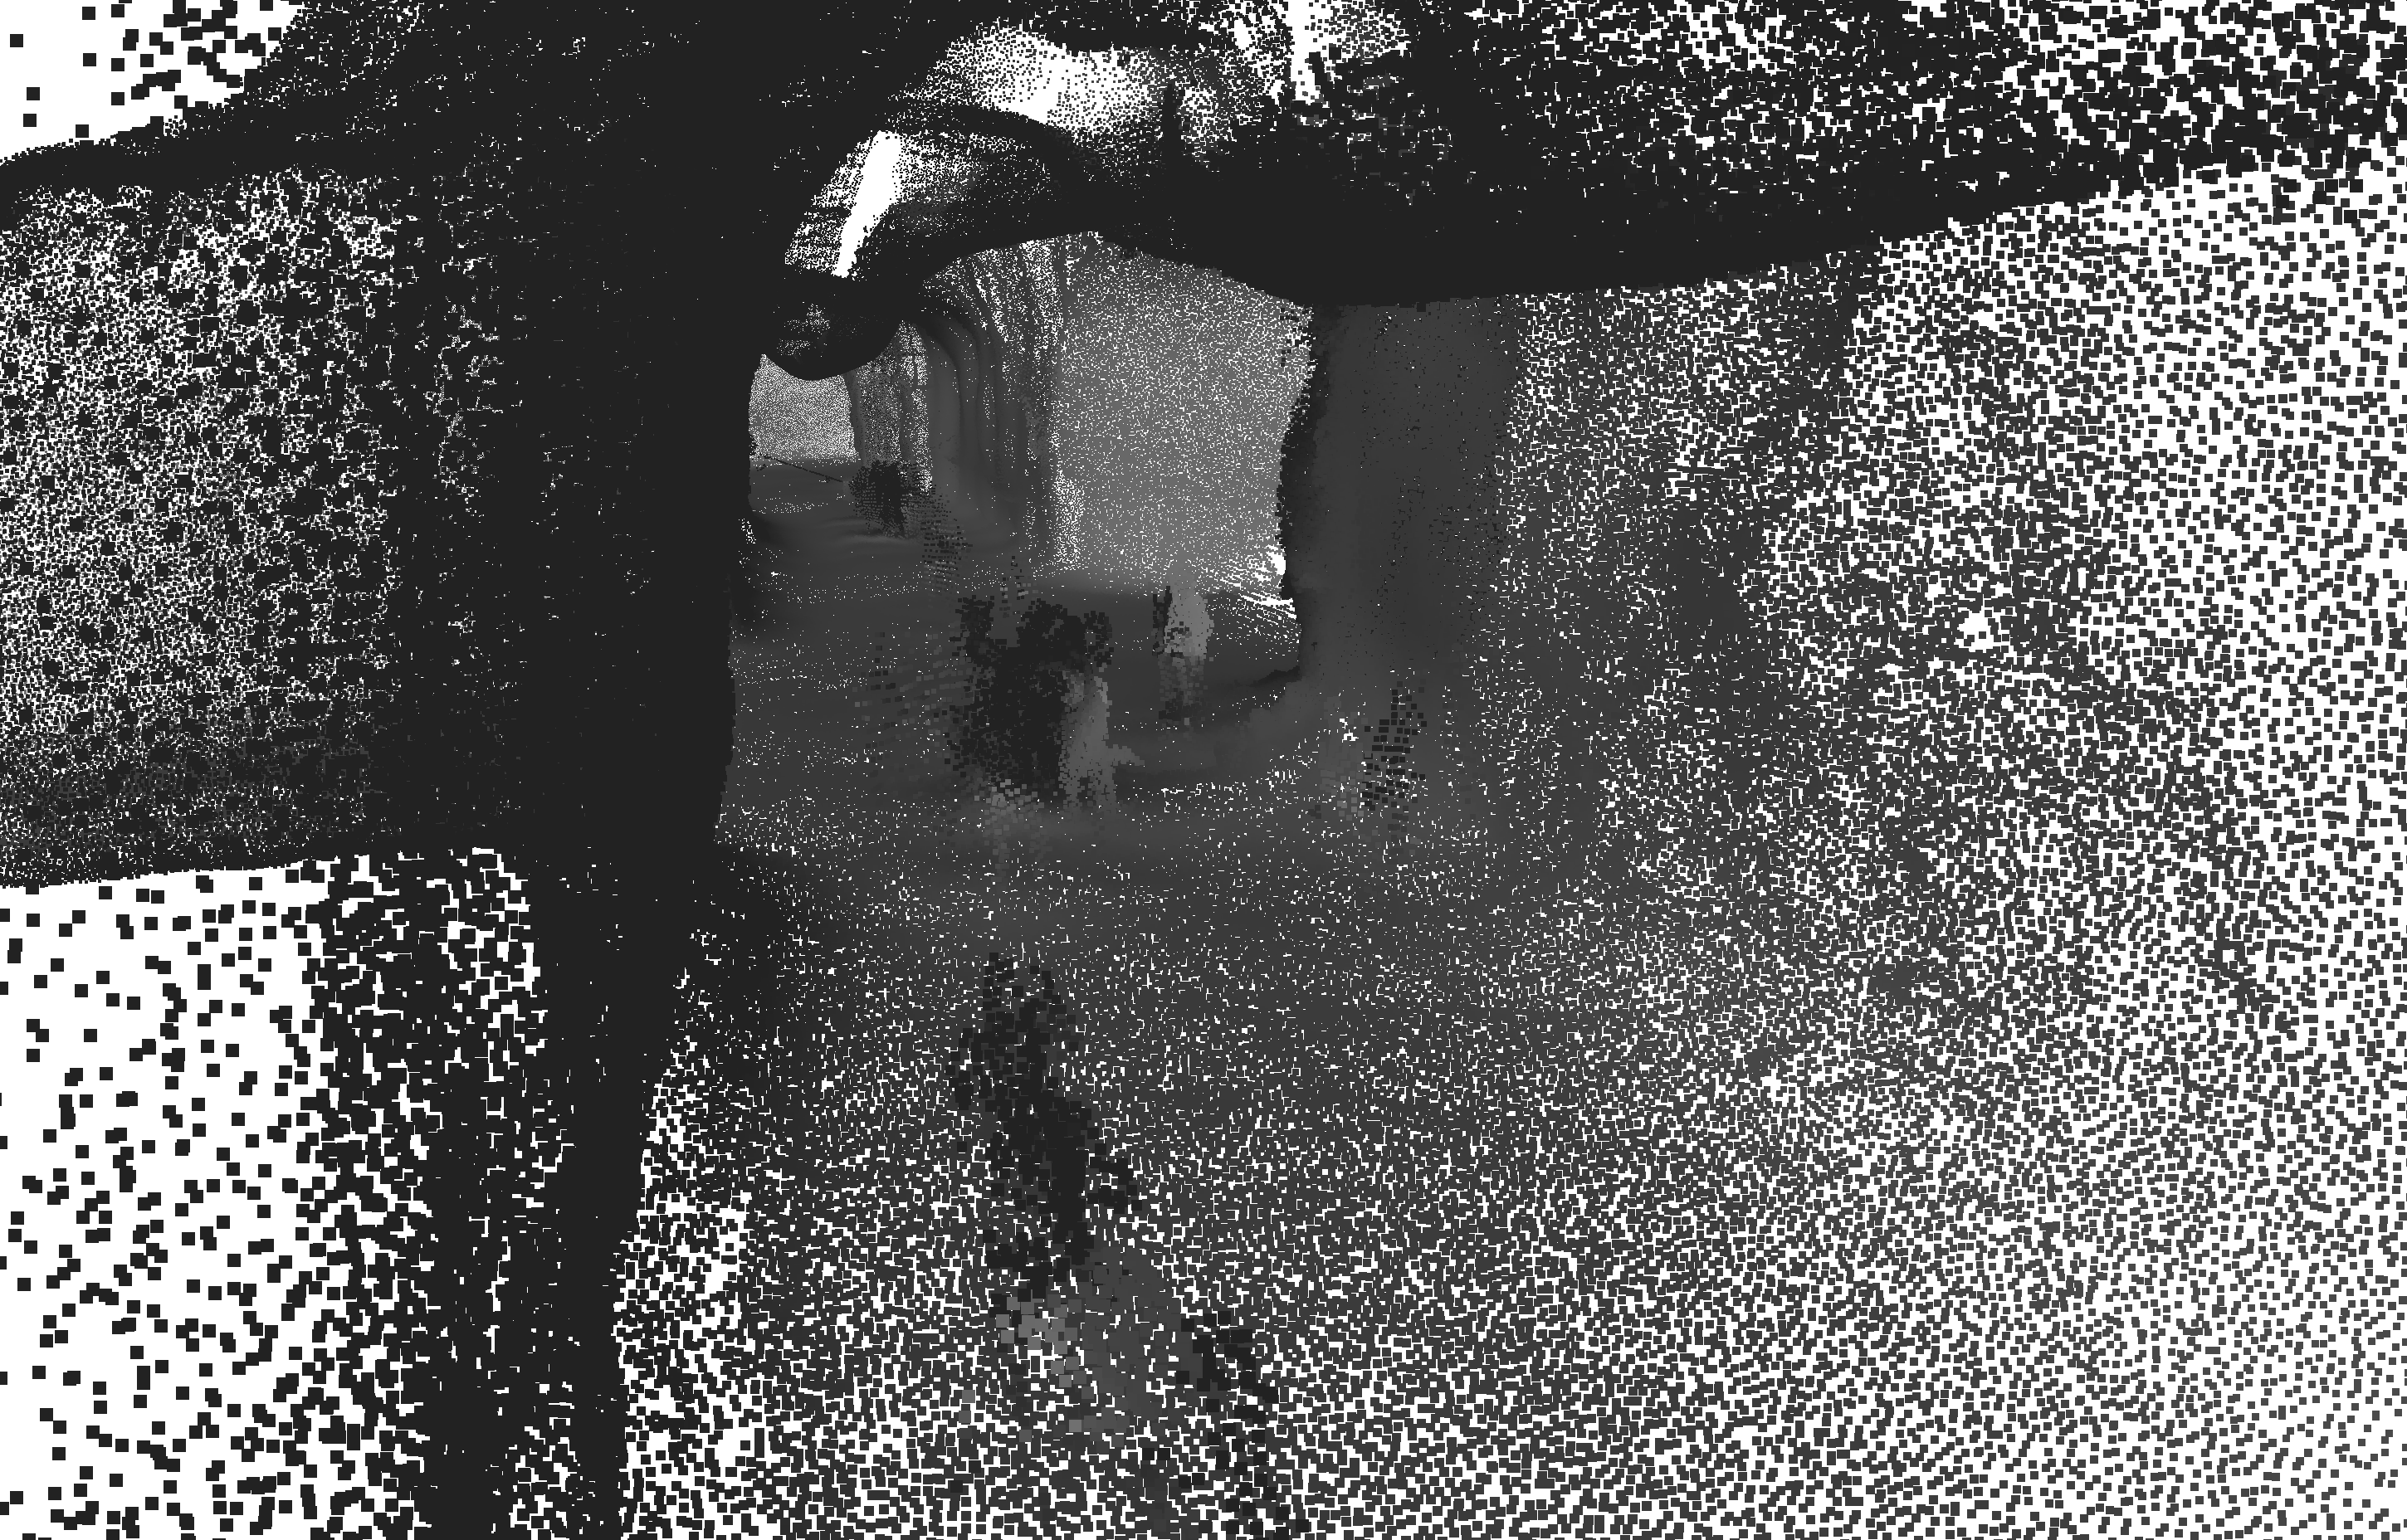
\includegraphics[width=0.95\linewidth]{closed_points}		
		Input set of points
	\end{minipage}%
	\hfill
	\begin{minipage}{0.5\linewidth}
		\centering
		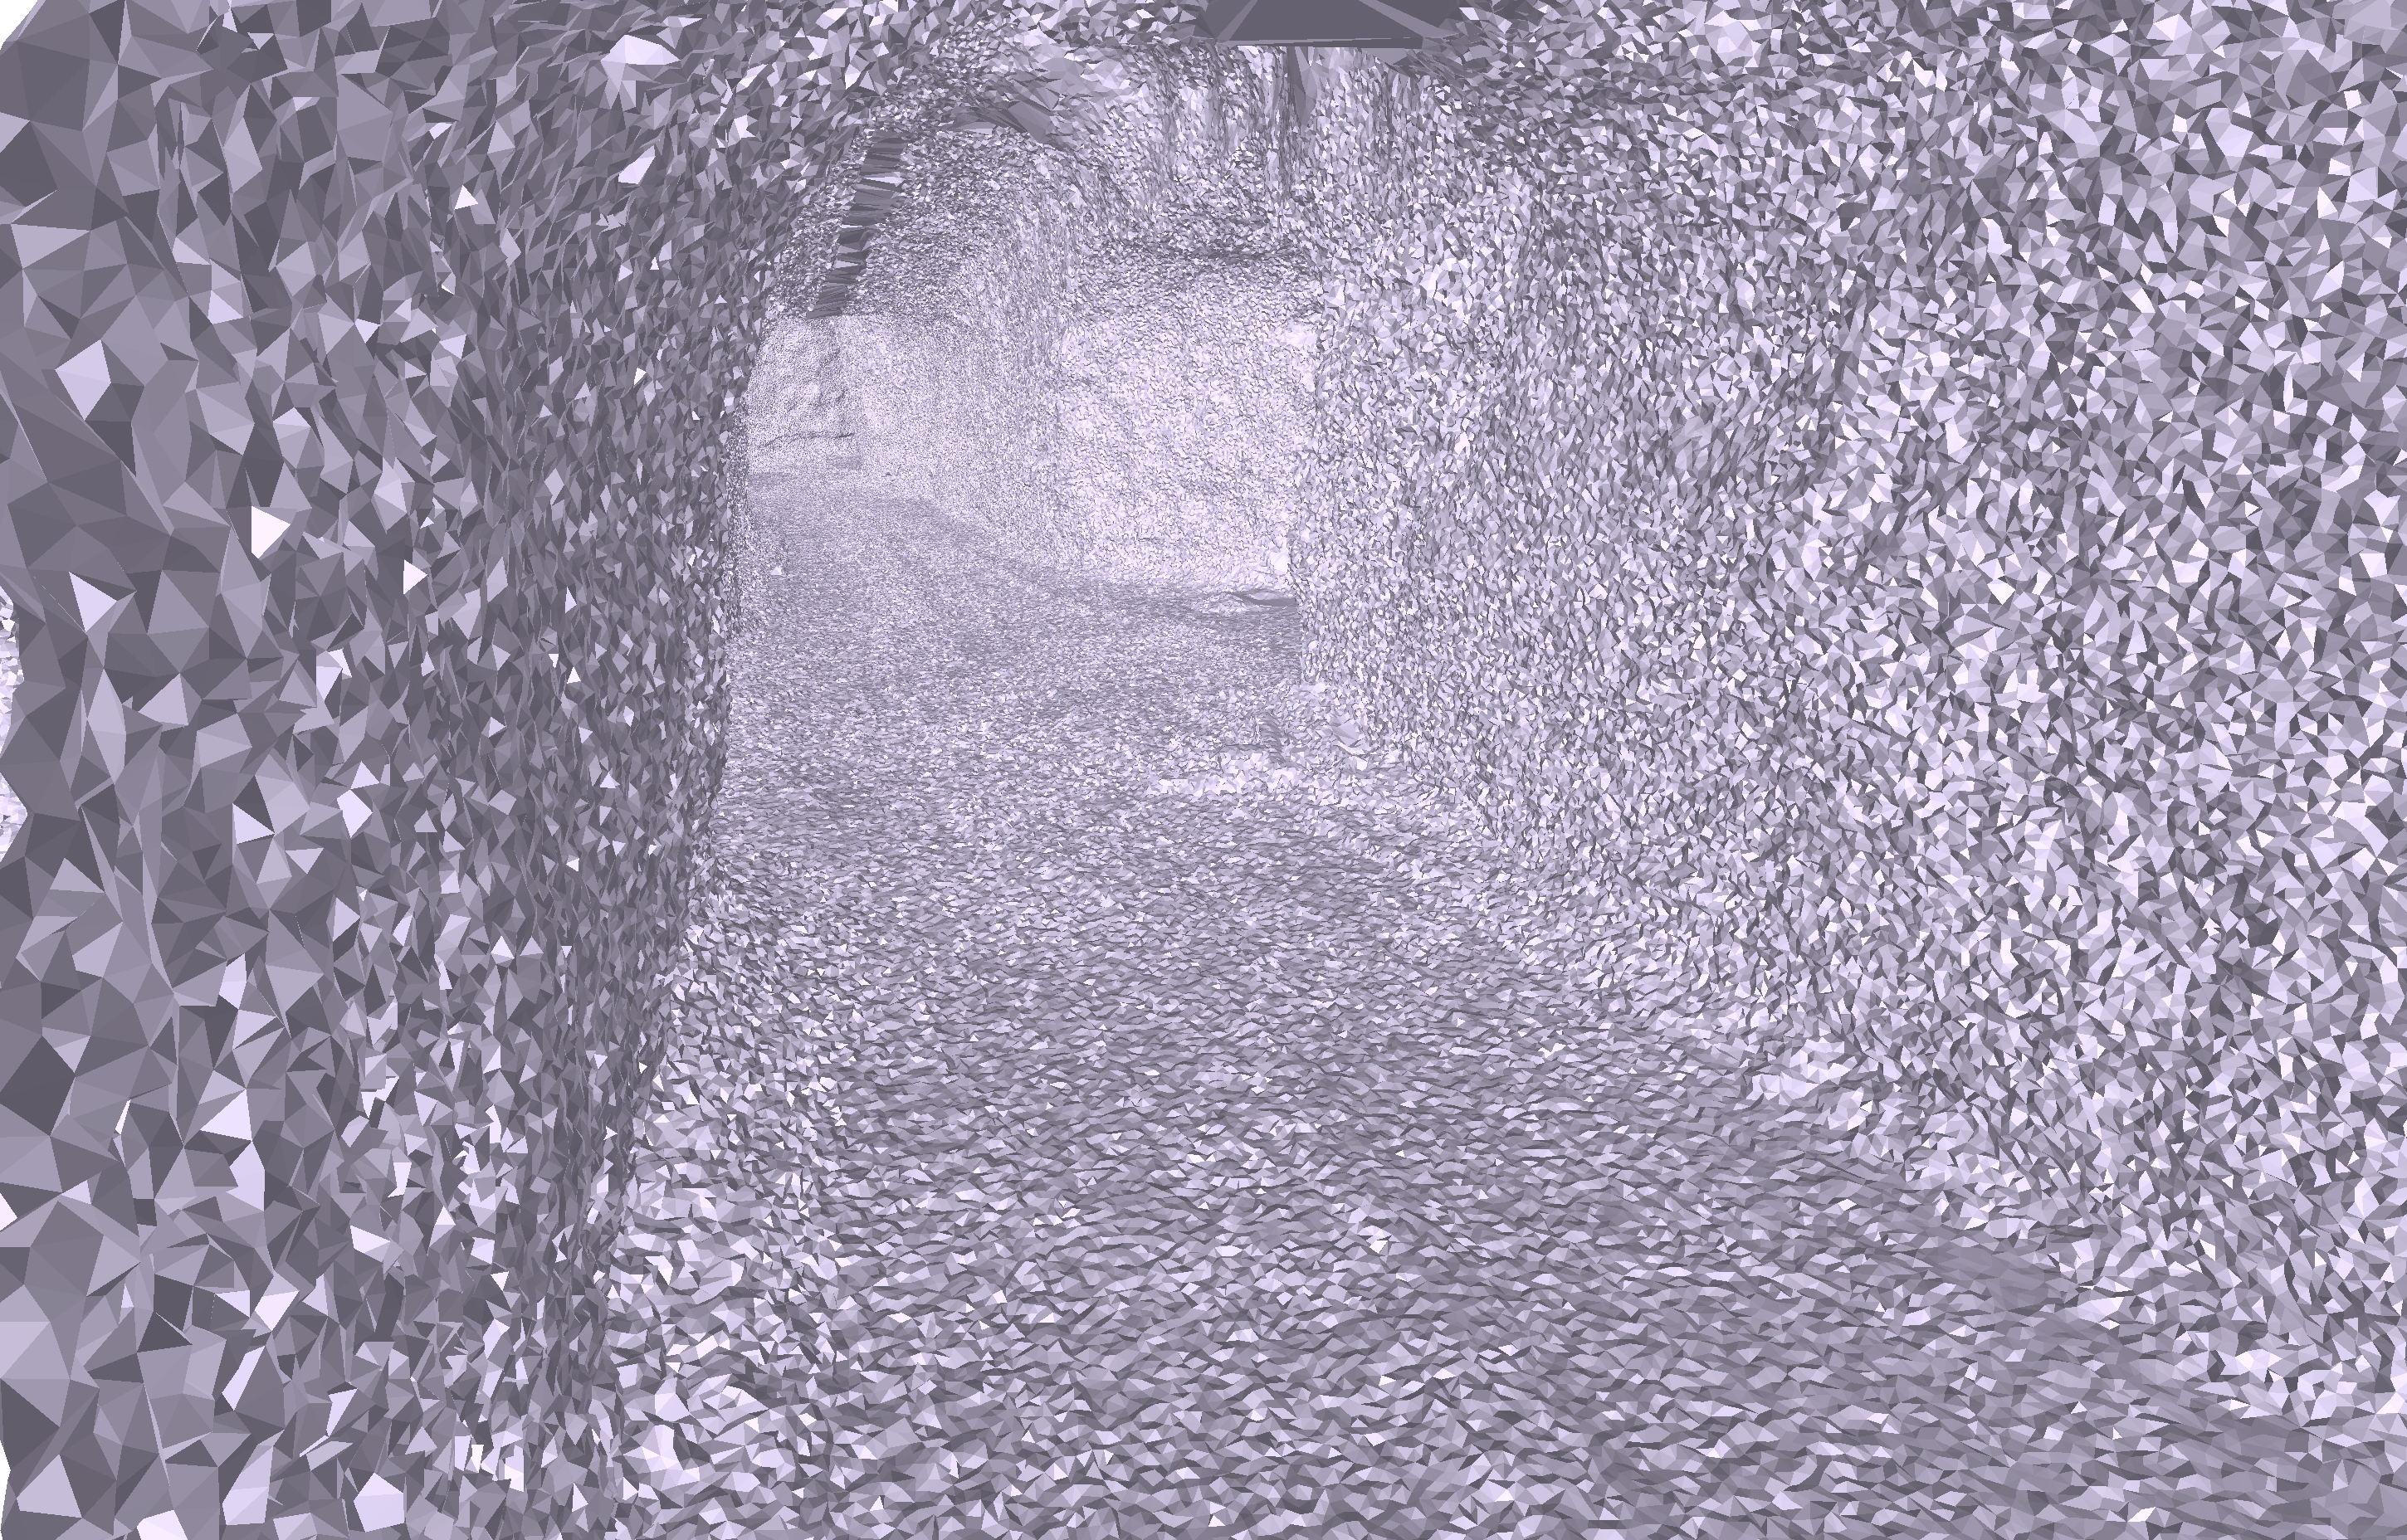
\includegraphics[width=0.95\linewidth]{closed_lex}	
		Lexicographic optimal cycle
	\end{minipage}
	
	\begin{minipage}{0.5\linewidth}
		\centering
		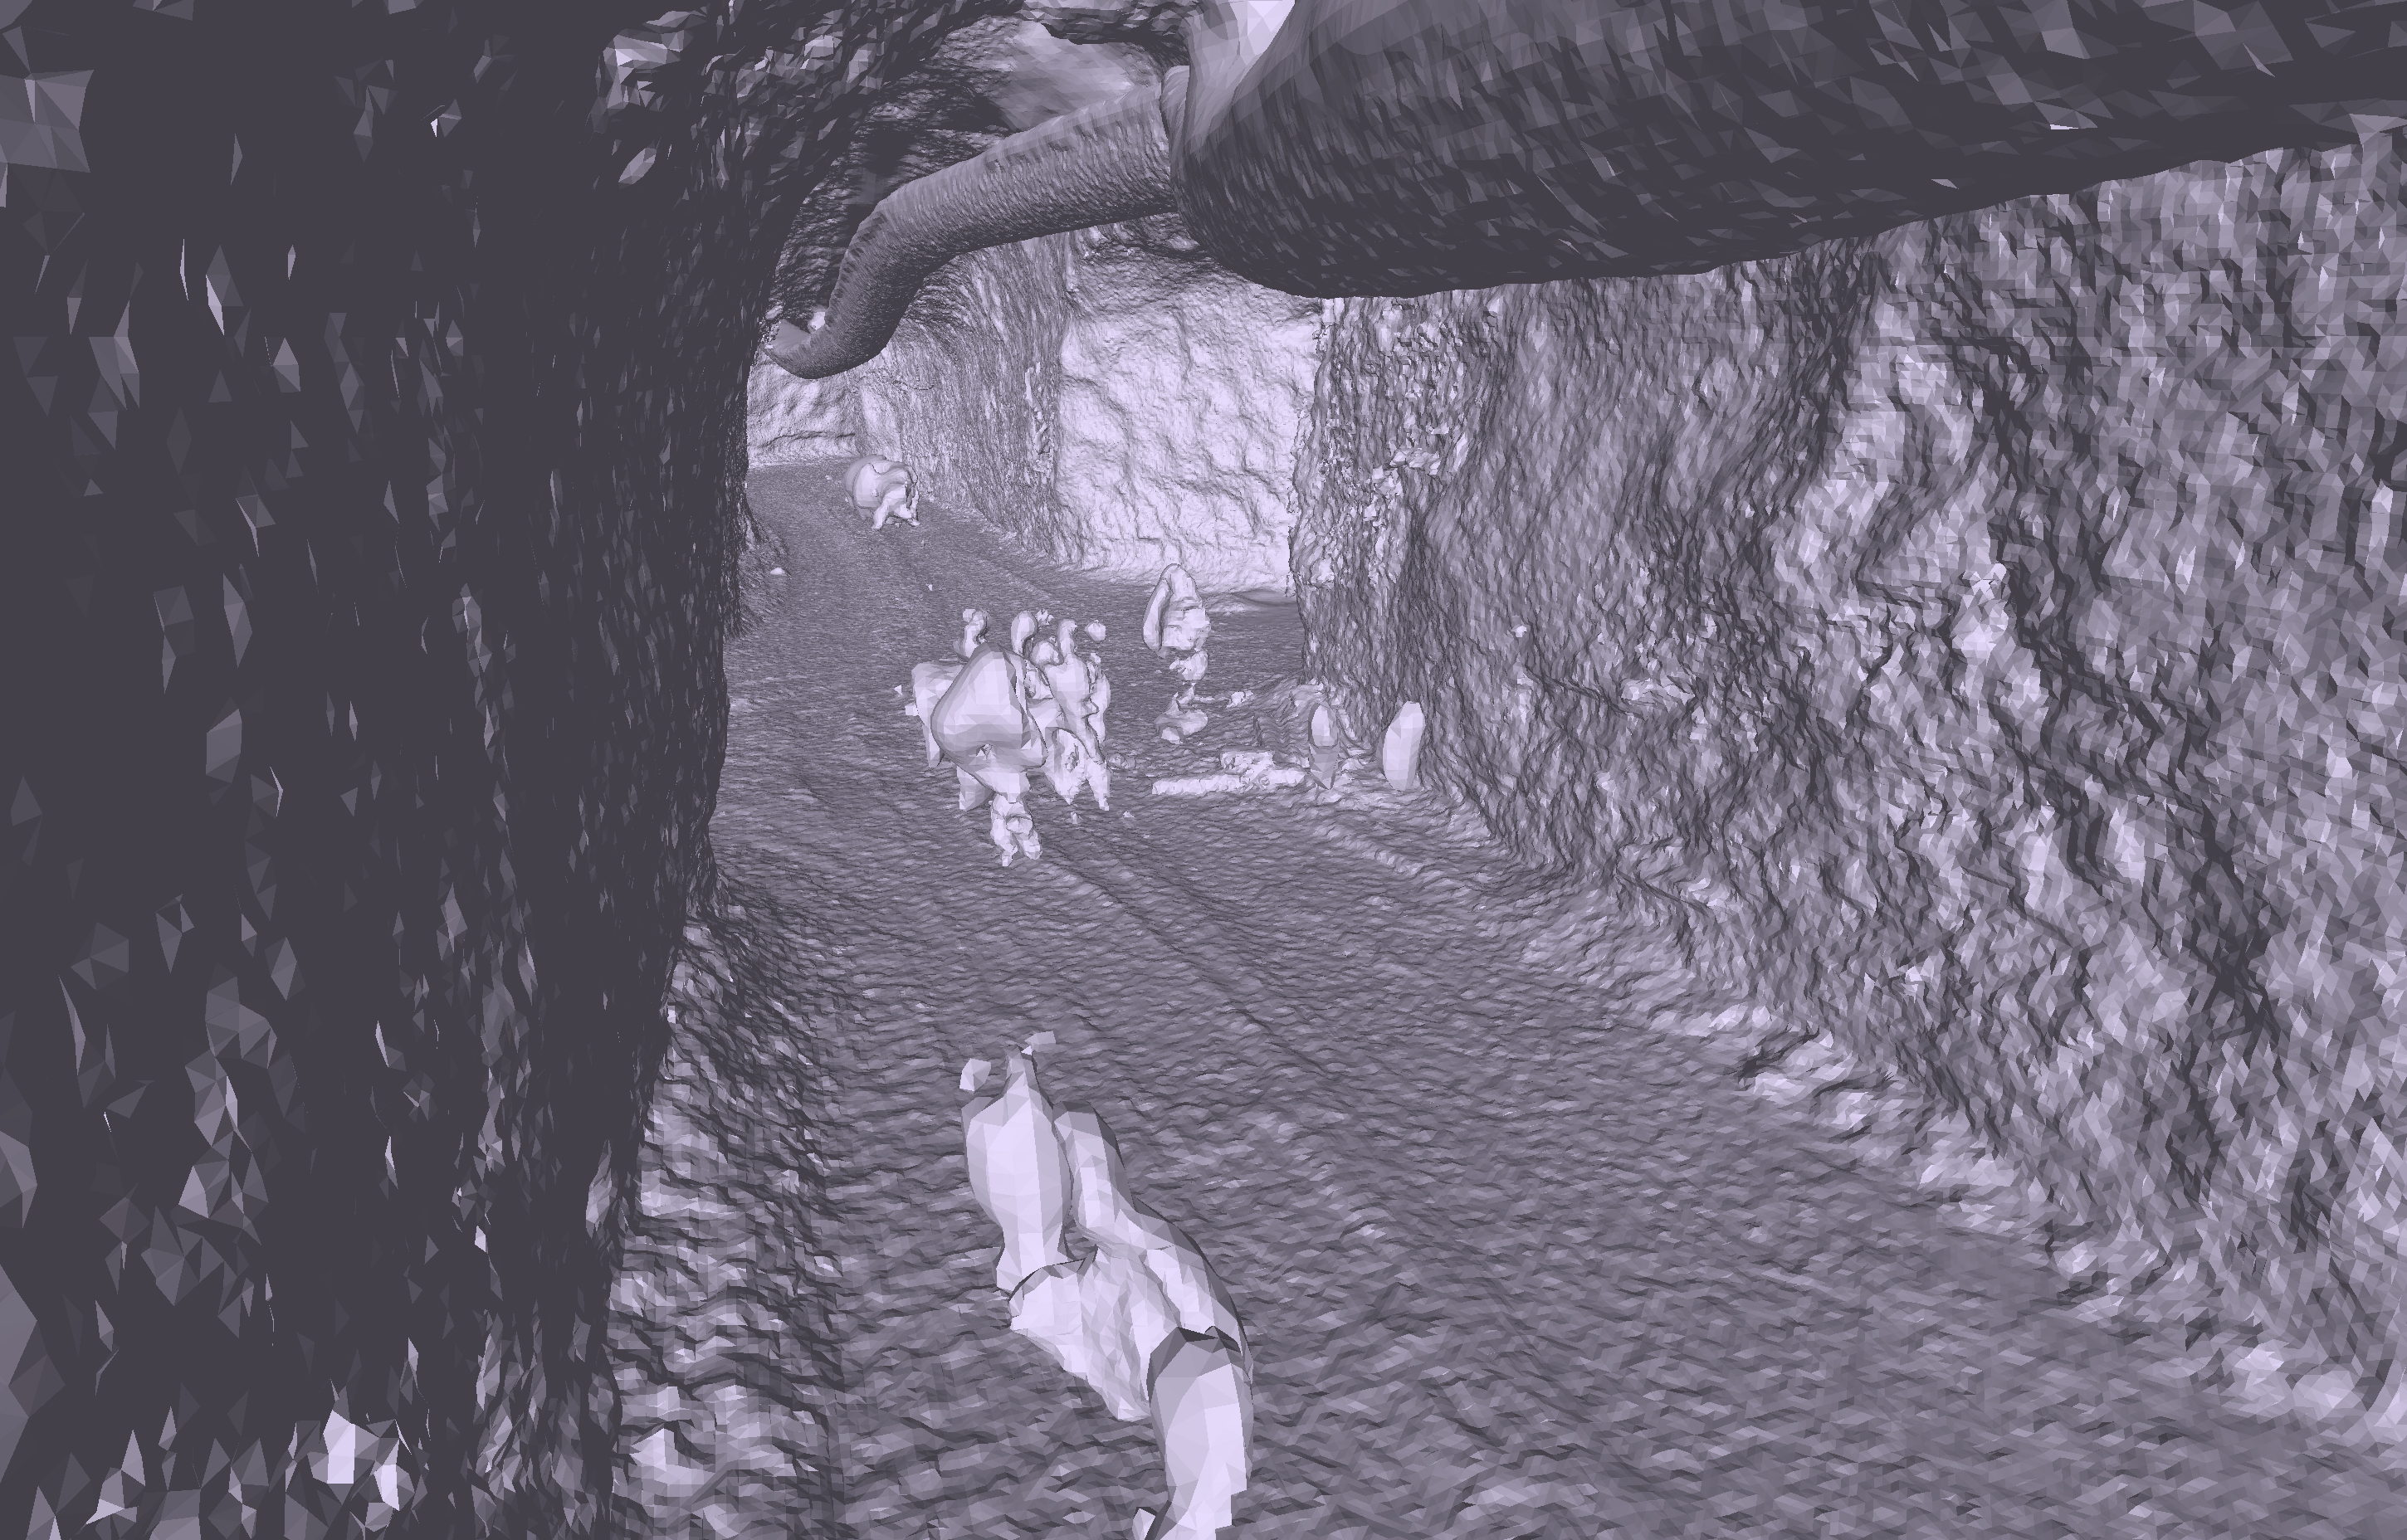
\includegraphics[width=0.95\linewidth]{closed_poisson}	
		Poisson reconstruction
	\end{minipage}%
	\begin{minipage}{0.5\linewidth}
		\centering
		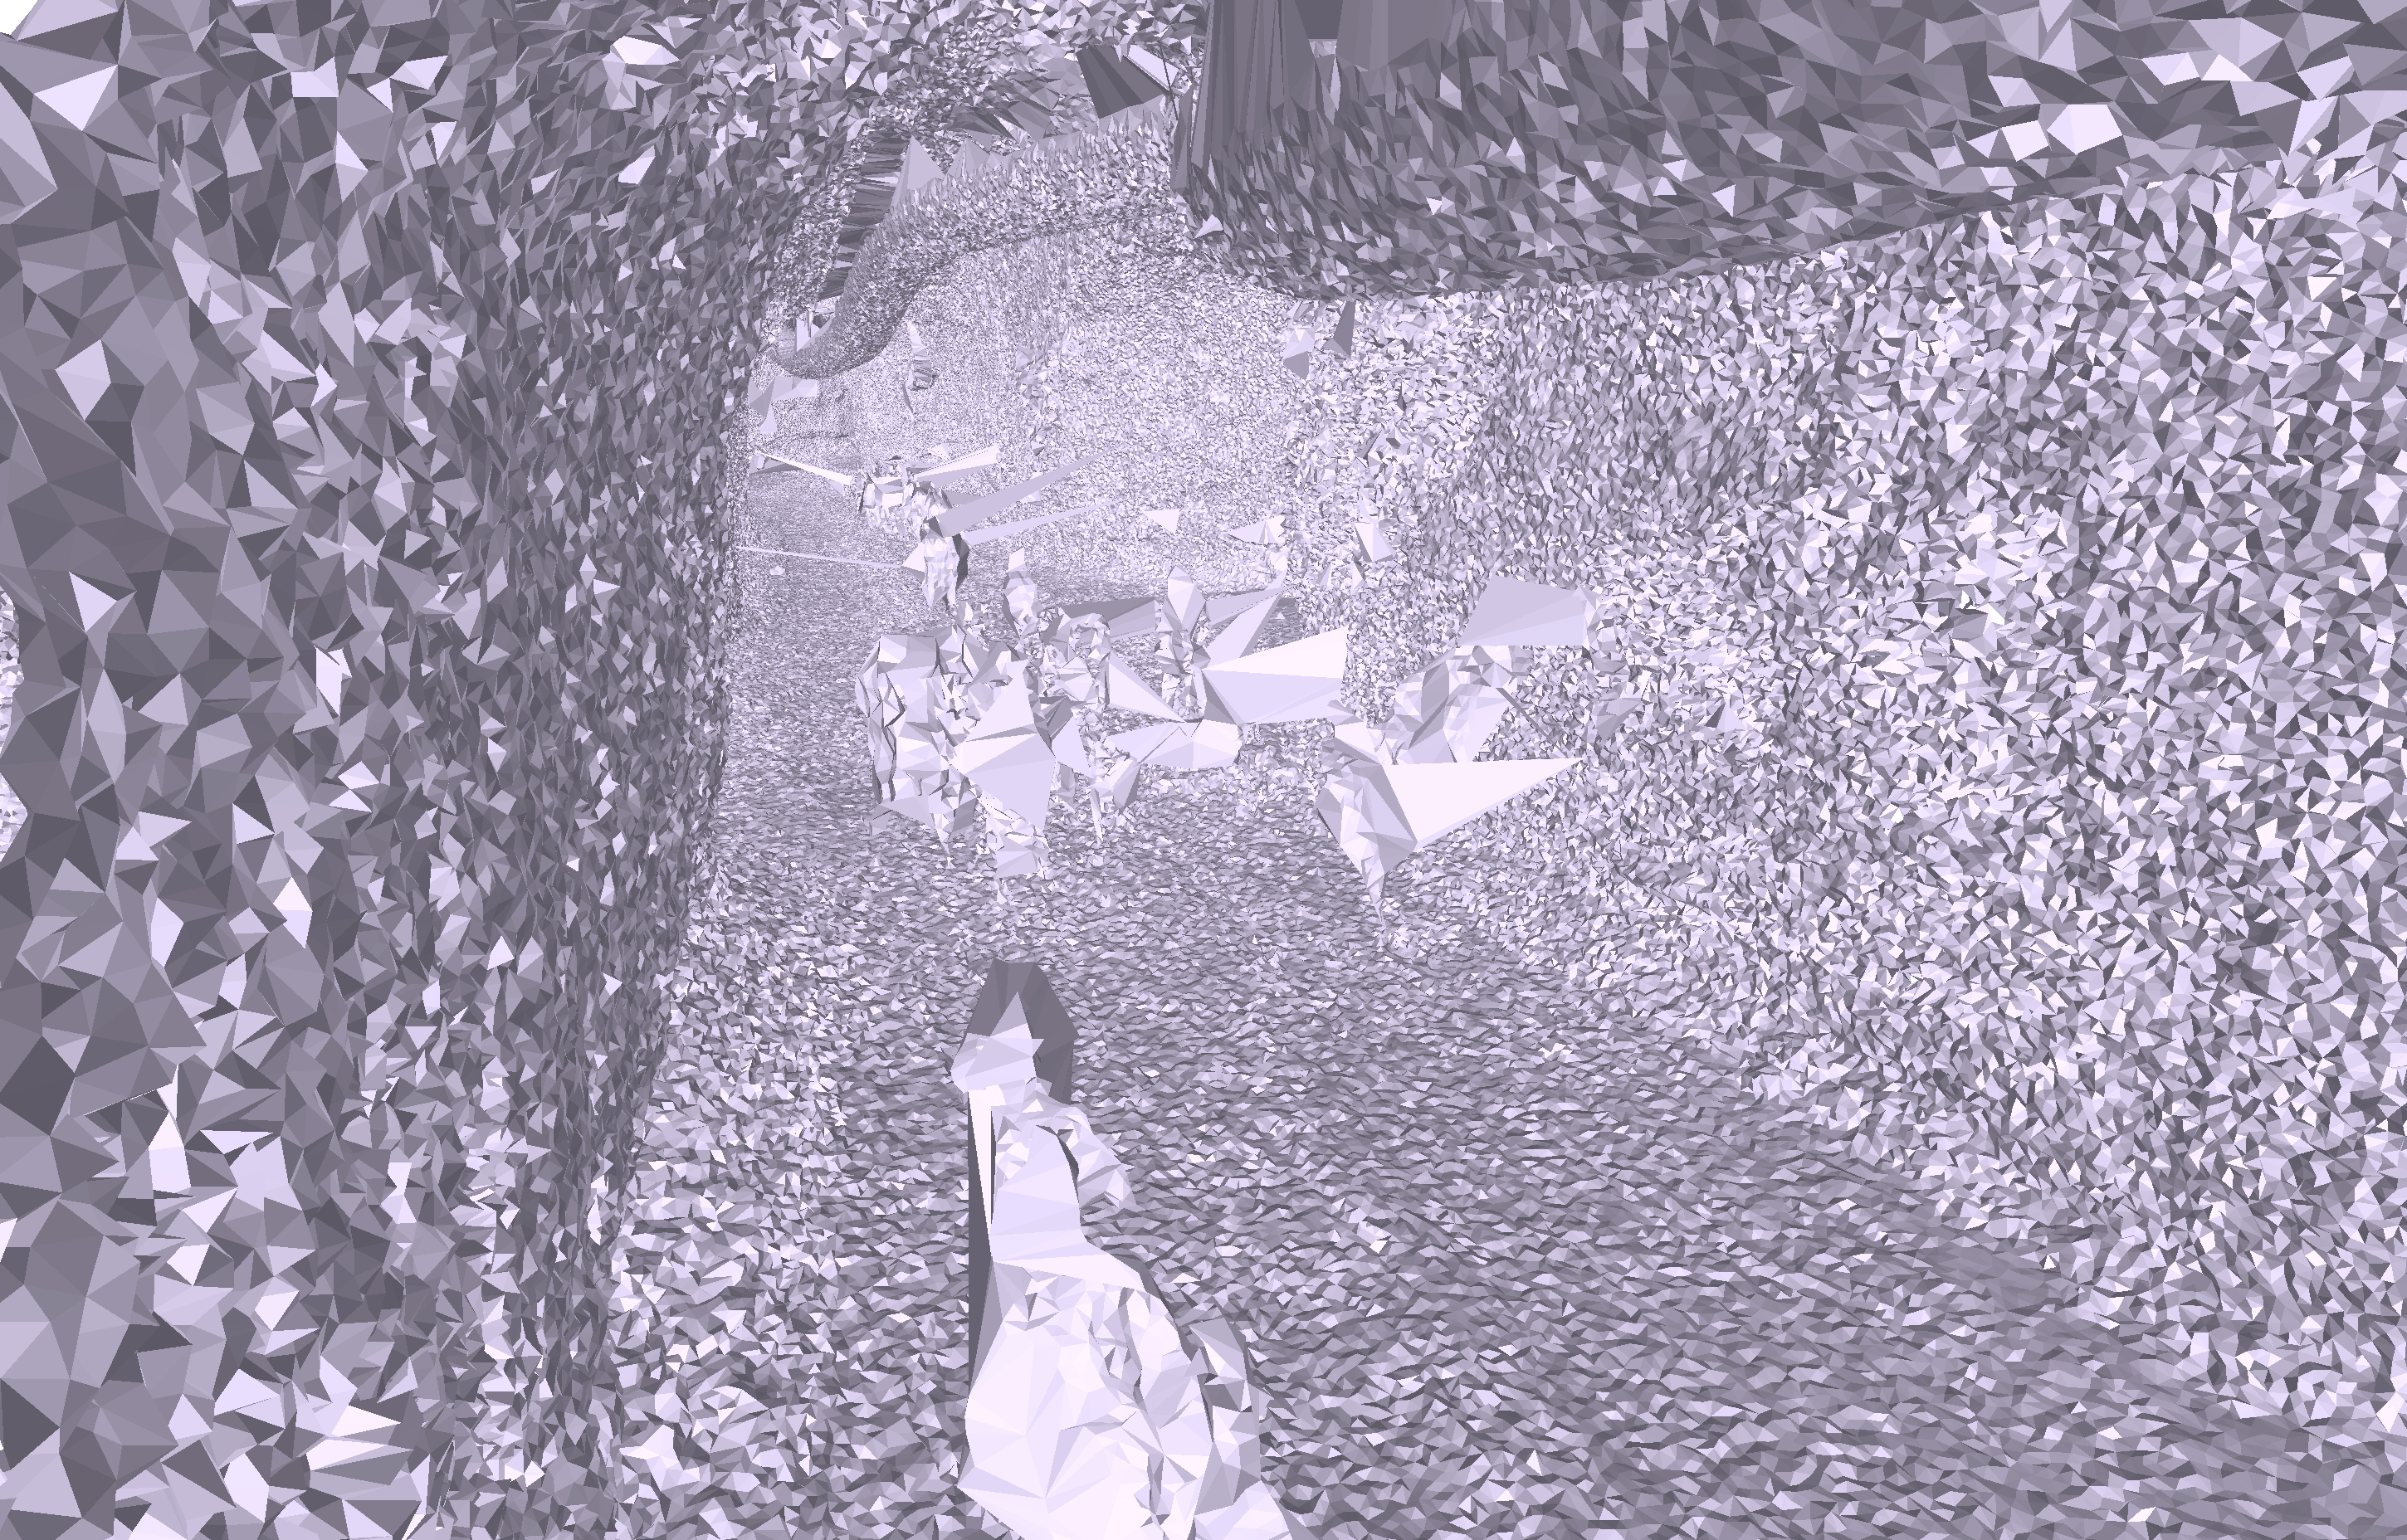
\includegraphics[width=0.95\linewidth]{closed_scalespace}	
		Advancing front reconstruction
	\end{minipage}
\end{frame}

\begin{frame}{Influence of topological information}
	\scriptsize
	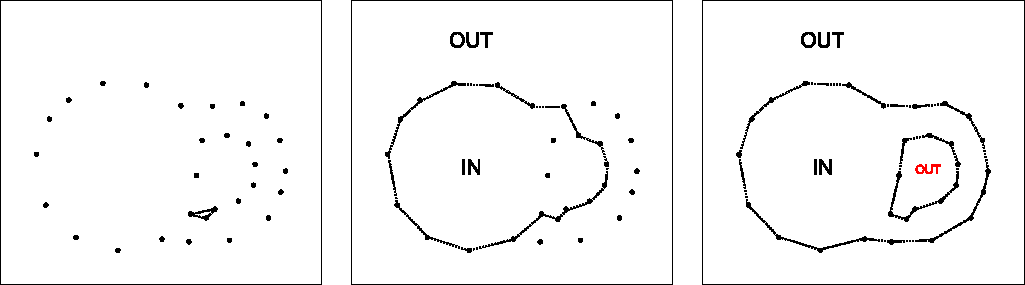
\includegraphics[width=\linewidth]{discovering_handle}
	\begin{tabularx}{\linewidth}{@{}YYY@{}}
		Global lexicographic cut & Single set of constraints & Additional constraints
	\end{tabularx}
\end{frame}

\begin{frame}{Theoretical guarantees}
	\scriptsize
	For a Čech or Vietoris-Rips complex, under very strict conditions linking the point set sampling, the parameter of the complex and the reach of the underlying manifold of Euclidean space, the minimal lexicographic chain in the fundamental class of the complex using the described simplex order is a triangulation of the sampled manifold \cite{cohen-steiner_LexicographicOptimalChains_2019}.
	
	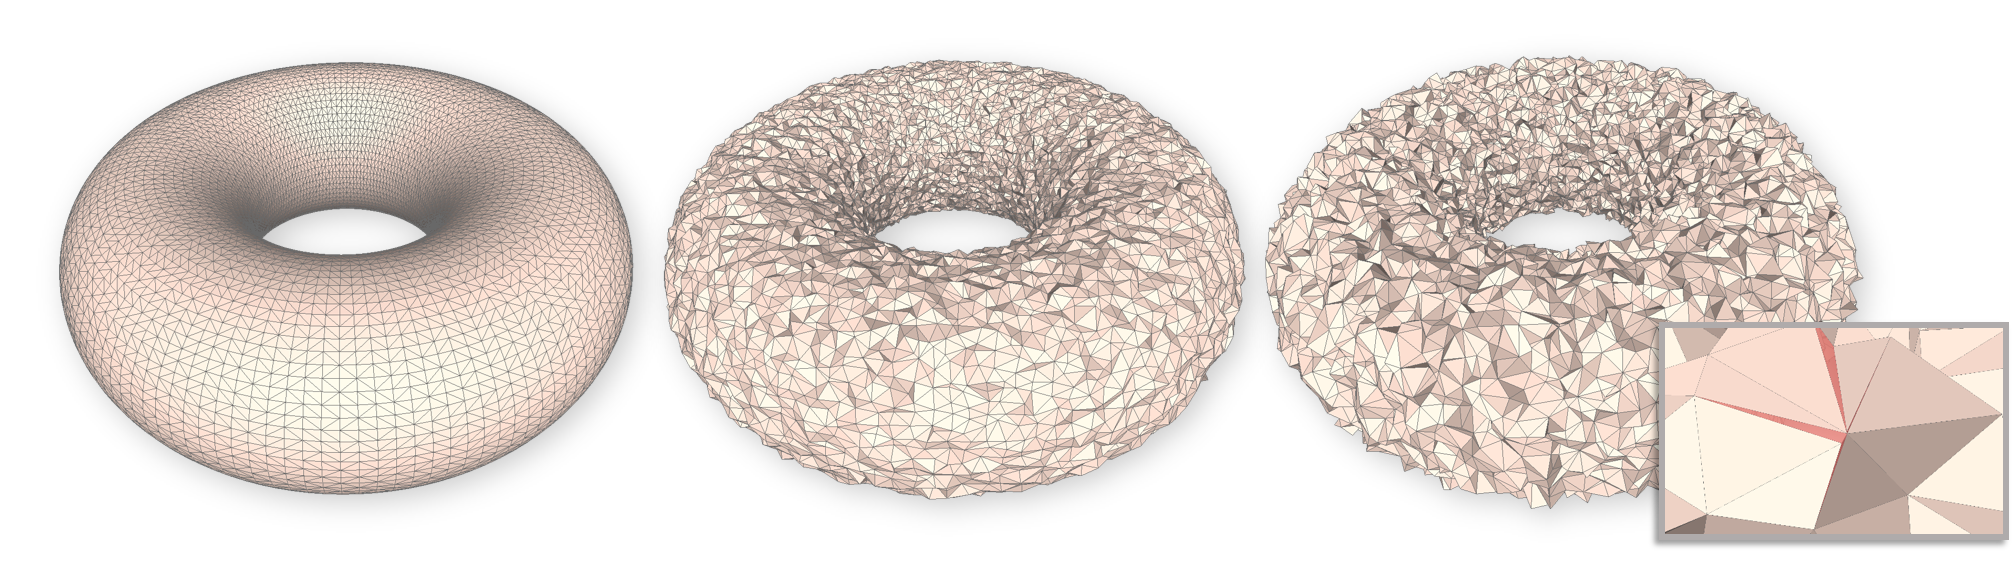
\includegraphics[width=\linewidth]{torus_3}	
\end{frame}

\begin{frame}{Spatial decomposition}
	\textbf{Tiling strategy} for large point clouds
	\begin{center}
		\includegraphics[width=0.45\linewidth]{dublin_parts}
		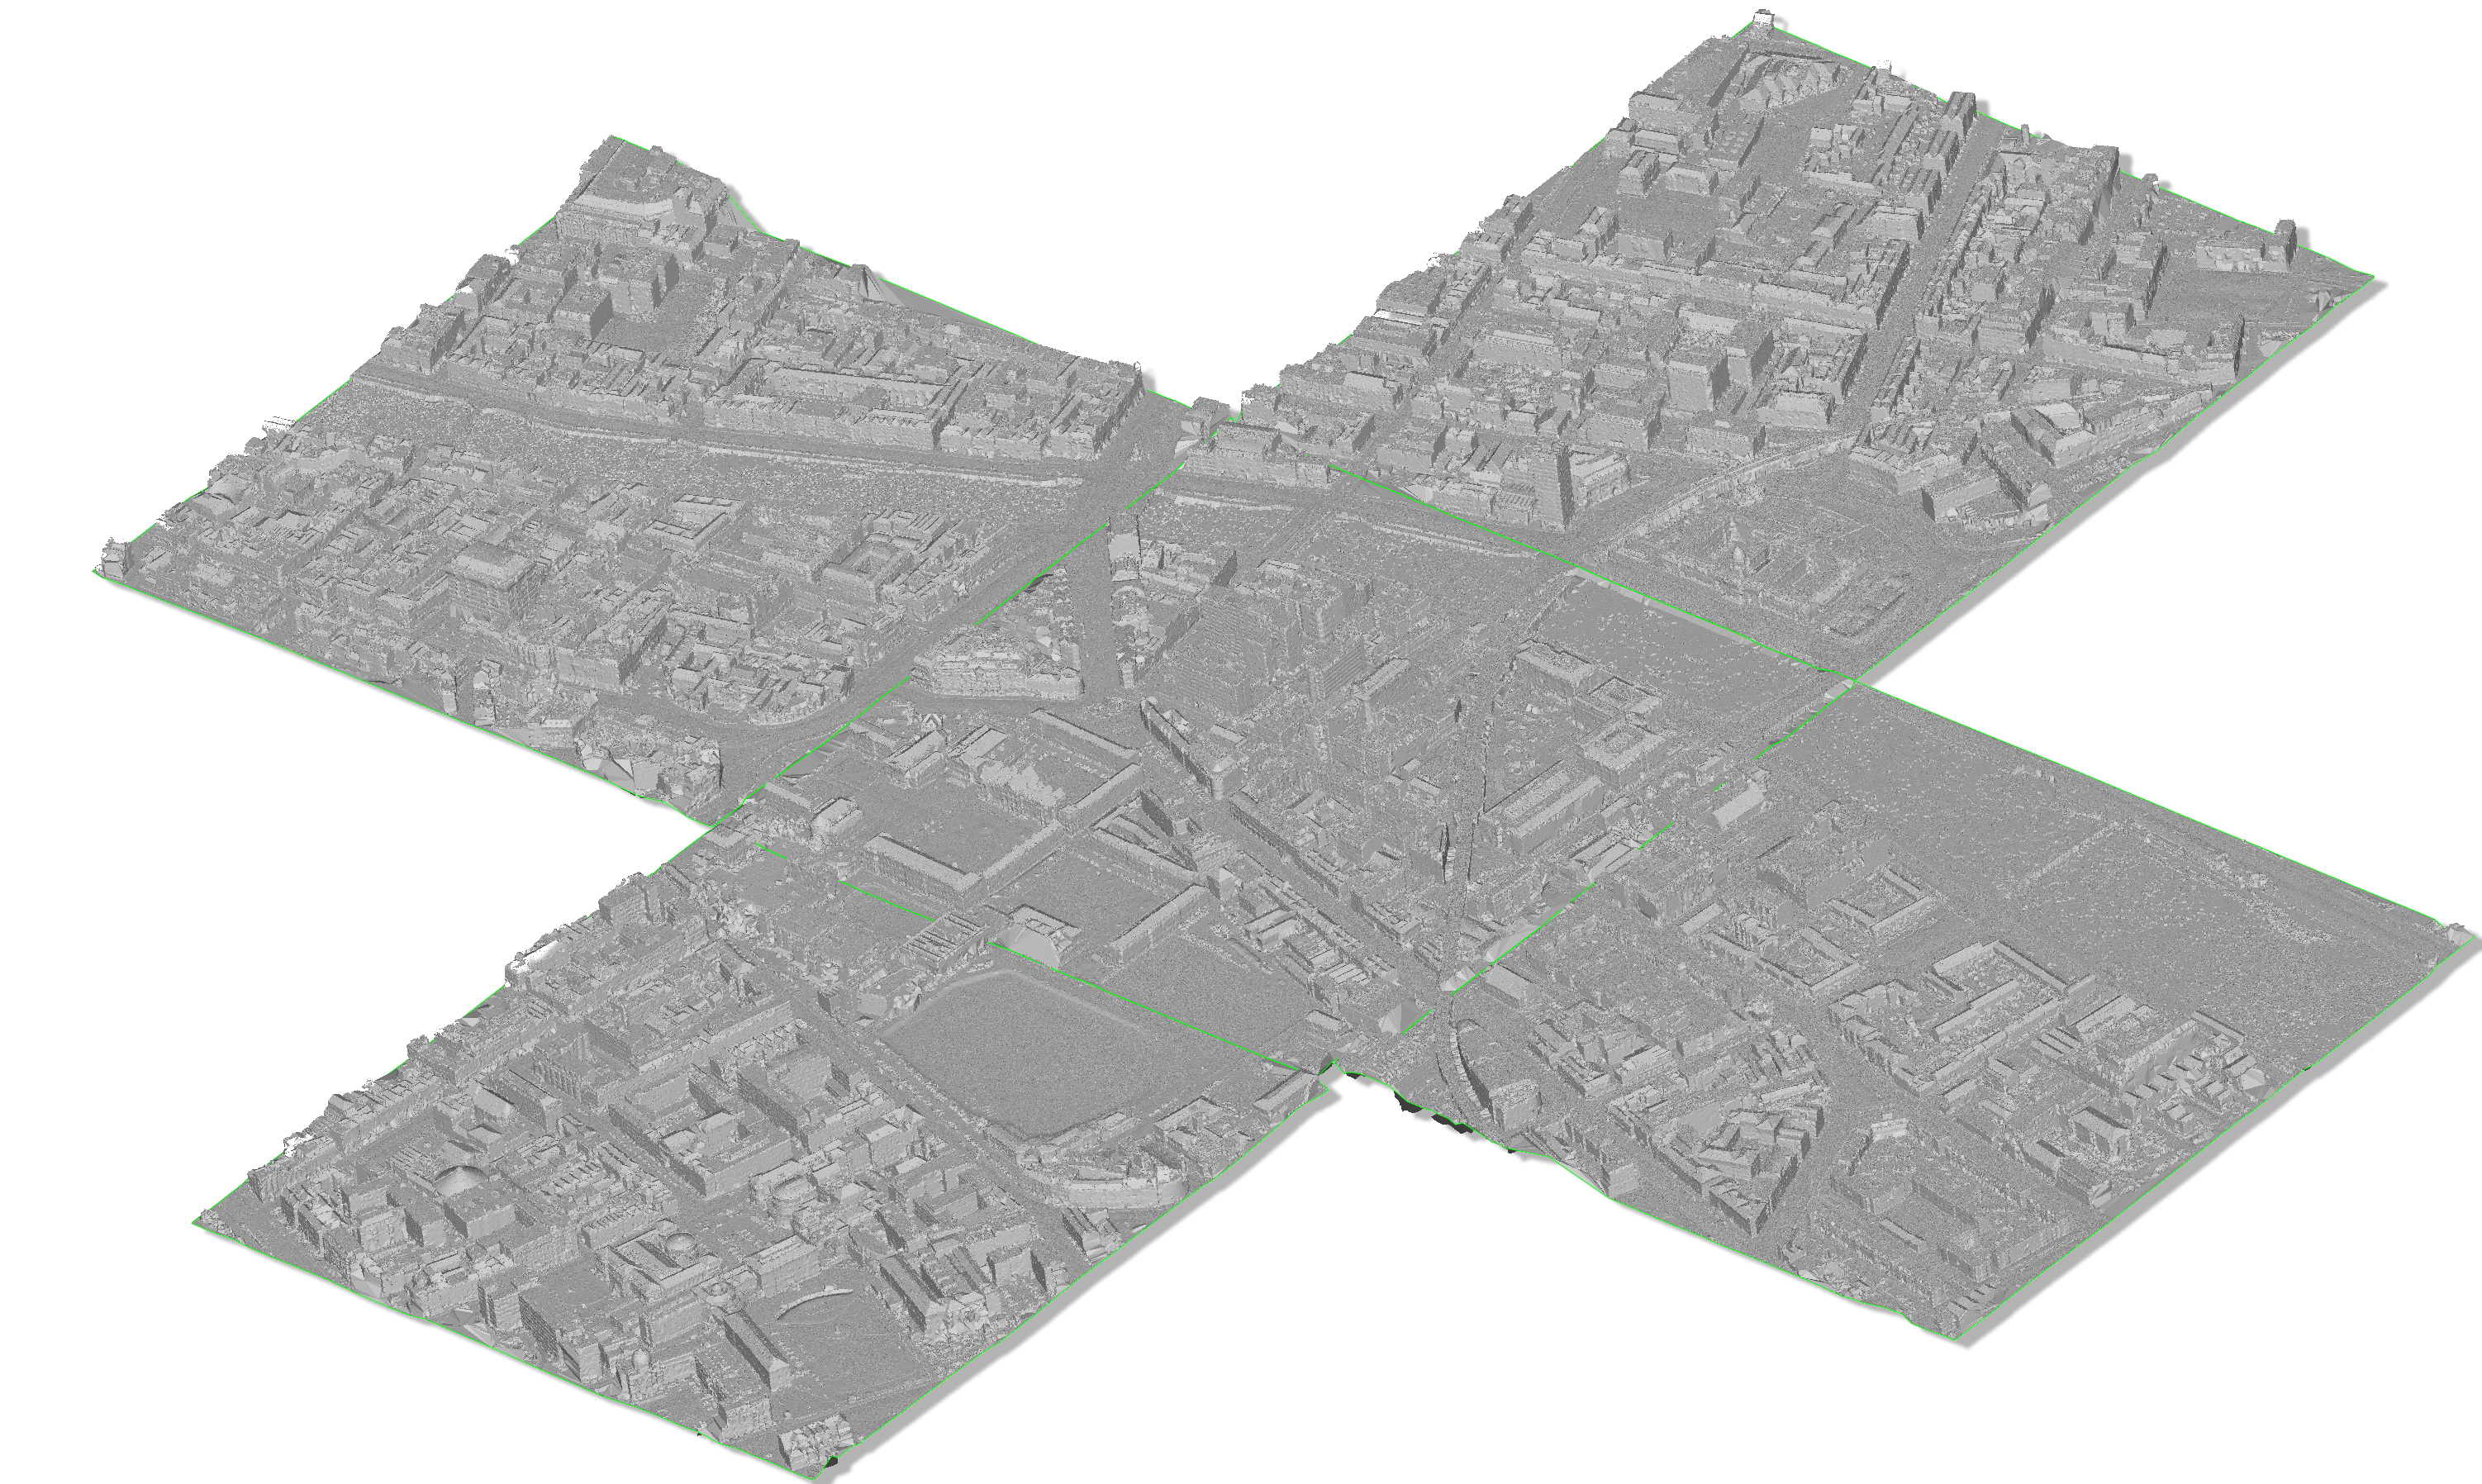
\includegraphics[width=0.45\linewidth]{terrain_multipart}
	\end{center}
\end{frame}
